\section{Powertrain Operating Point}
\label{power_train_op_point}
In these notes, we are not particularly interested in how the combustion engine operates. In contrast, we are interested in automobiles as a macroscopic system that we would
like to understand and control. In this context, we will treat the combustion engine (or any other means whatsoever producion the propulsion force) as a black box.
However, we want to be able to argue upon how much force the engine system should produce such that the vehicle is able to accelerate, decelerate or travel at constant speed.
In this chapter therefore, we will introduce the basic physical laws that govern the motion of the vehicle. In particular, we will consider

\begin{itemize}
\item Longitudinal vehicle dynamics
\item Aerodynamic force $\mathbf{F}_{aero}$
\item Rolling force $\mathbf{F}_{roll}$
\item Gravitational force $\mathbf{F}_{grav}$
\end{itemize}

By considering the above mentioned forces, we will be able to produce a basic model that explains the longitudinal dynamics of the vehicle. In chaper \ref{model_automotive_sys} we will get more into modeling the subsystems of the vehicle and come up with a more refined model.


\section{Aerodynamics \& Rolling Resistance}

Let us start simple and assume the motion of a vehicle in a flat road; no road gradietns. There are three types of forces that are always present in such a scenario; the propulsion force, $\mathbf{F}_{p}$, produced by the  powertrain, the rolling force $\mathbf{F}_{roll}$ produced by the friction of the tires and the road and the aerodynamic force  $\mathbf{F}_{aero}$ which is caused due to the motion of the vehicle in the air. We can see schematically how these forces act in figure \ref{flat_road_vehicle_diagram}

\begin{figure}[!htb]
\begin{center}
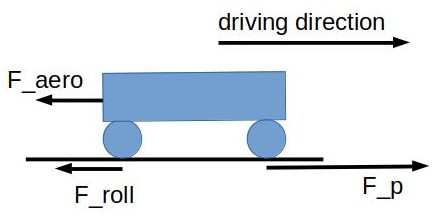
\includegraphics[scale=0.280]{img/physics/flat_road_vehicle_diagram.jpg}
\end{center}
\caption{Schematics of longitudinal forces acting on vehicle.}
\label{flat_road_vehicle_diagram}
\end{figure}

\begin{framed}

\textbf{Remark}

In figure \ref{flat_road_vehicle_diagram}, the vectors have not been drawn to scale. Also, the propulsion force $\mathbf{F}_{p}$ is applied to every motorised wheel however, for simplicity we consider the net or total propulsion force acting on the vehicle. Similarly, the rolling force $\mathbf{F}_{roll}$ represents the total rolling force and not the individual force acting on every wheel. Finally, and in the same vein, the aerodynamic force, $\mathbf{F}_{aero}$,  is the total force acting on the vehicle.

\end{framed}

\begin{framed}

\textbf{Remark}

Forces in the other directions mainly affect the suspension and the steering of the vehicle and we will not consider them here.

\end{framed}

It is easy to understand that $\mathbf{F}_{roll}$ will be zero when the vehicle is not moving. A commonly used model is:


\begin{equation}
\mathbf{F}_{roll}(\alpha) = \left\{
\begin{array}{rl}
	0 & \text{if } v = 0,\\
	\pm c_rmg\cos(\alpha) & \text{if } v \neq 0 
\end{array} \right.
\end{equation}

where 

\begin{itemize}
\item $\alpha$ is the road slope
\item $m$ is the vehicle mass
\item $c_r$ is the rolling resistance coefficient. Typically, is about 0.01 
\item $g$ is the gravitational acceleration constant
\end{itemize}

The rolling resistance force, is approximately independent of the vehicle speed and it exhibits some variation with respect to the road angle. It acts in the opposite direction of the
driving. Thus, it changes sign if the vehicle is moving in the reverse direction. $c_r$ should be as small as possible in order to keep the energy consumption low. 


\section{Questions}


\textbf{Question 1}

Suppose a vehicle is coasting on a flat road, that is, there are no propelling or braking forces acting on the vehicle. This means the only forces that are acting on the vehicle are the rolling resistance and aerodynamic forces. Below you find diagrams describing those forces as a function of vehicle speed

\begin{figure}[!htb]
\begin{center}
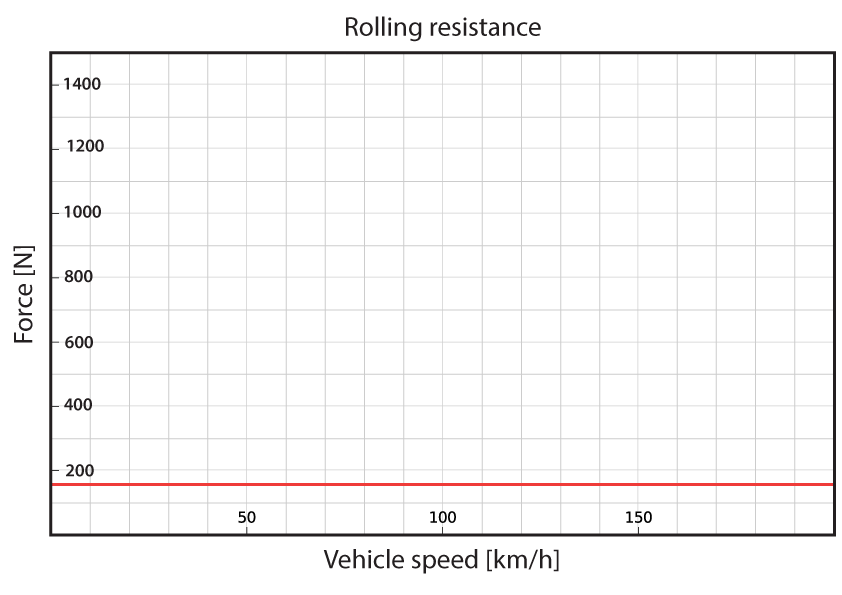
\includegraphics[scale=0.280]{img/model_automotive_sys/Diagram_RollingResistance_01.png}
\end{center}
\caption{Rolling force diagram.}
\label{Diagram_RollingResistance_01}
\end{figure}

\begin{figure}[!htb]
\begin{center}
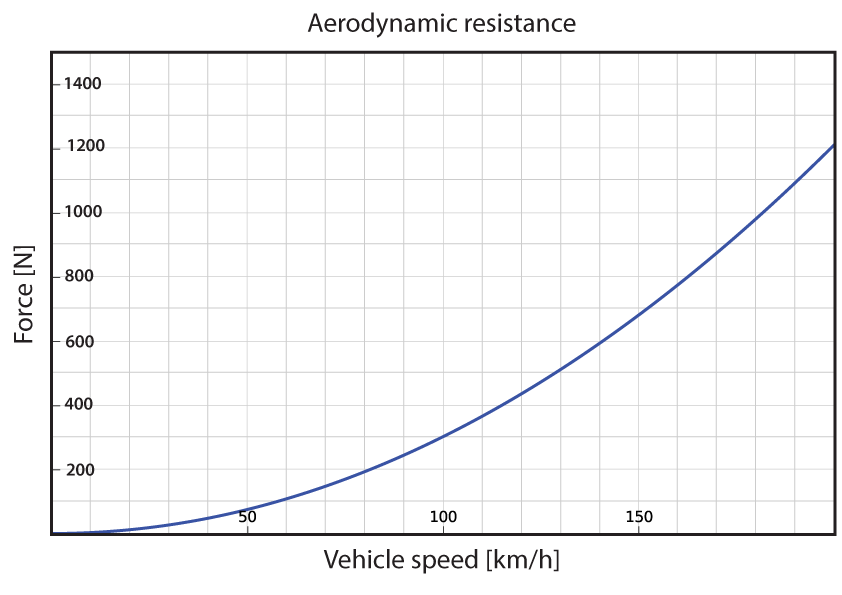
\includegraphics[scale=0.280]{img/model_automotive_sys/Diagram_AerodynamicResistance_01.png}
\end{center}
\caption{Aerodynamics force diagram.}
\label{Diagram_AerodynamicResistance_01}
\end{figure}

What is the sum of the rolling resistance and aerodynamic forces (N) at 100 km/h?


\textbf{Question 2}

Assume the vehicle in question 1 above has the following data:

\begin{tabular}{lll}
\hline
$m$ & 1600\\
$\alpha4$ & 0.0 \\
$A_f$ & 2.1\\
$c_r$ & 0.01\\
$C_D$ & 0.3 \\
$\rho$ & 1.25 \\
$g$ & 9.81 \\
\hline
\end{tabular}

What is the running resistance on a flat road, i e the sum of the rolling resistance and the aerodynamic resistance at 50 km/h? What is the running resistance on a flat road, i e the sum of the rolling resistance and the aerodynamic resistance at 150 km/h?

\textbf{Question 3}

Consider the same vehicle as in Ex.1-2 above. What happens to the resisting forces if the vehicle is made 50\% heavier, but all other parameters remain the same? If the  vehicle front area $A_f$ is increased 10\%, but all other parameters remain the same?







